% !TEX encoding = UTF-8 Unicode
% !TEX TS-program = xelatex

\documentclass[a4paper, 12pt]{book}

\usepackage{FDUThesis}
\usepackage{gbt7714} %在正文中 \cite 文献
\author{Yizhan Miao $<$\href{mailto:yzmiao@pm.me}{yzmiao@pm.me}$>$}

\begin{document}
\setlength{\baselineskip}{20pt}  % 20磅行间距
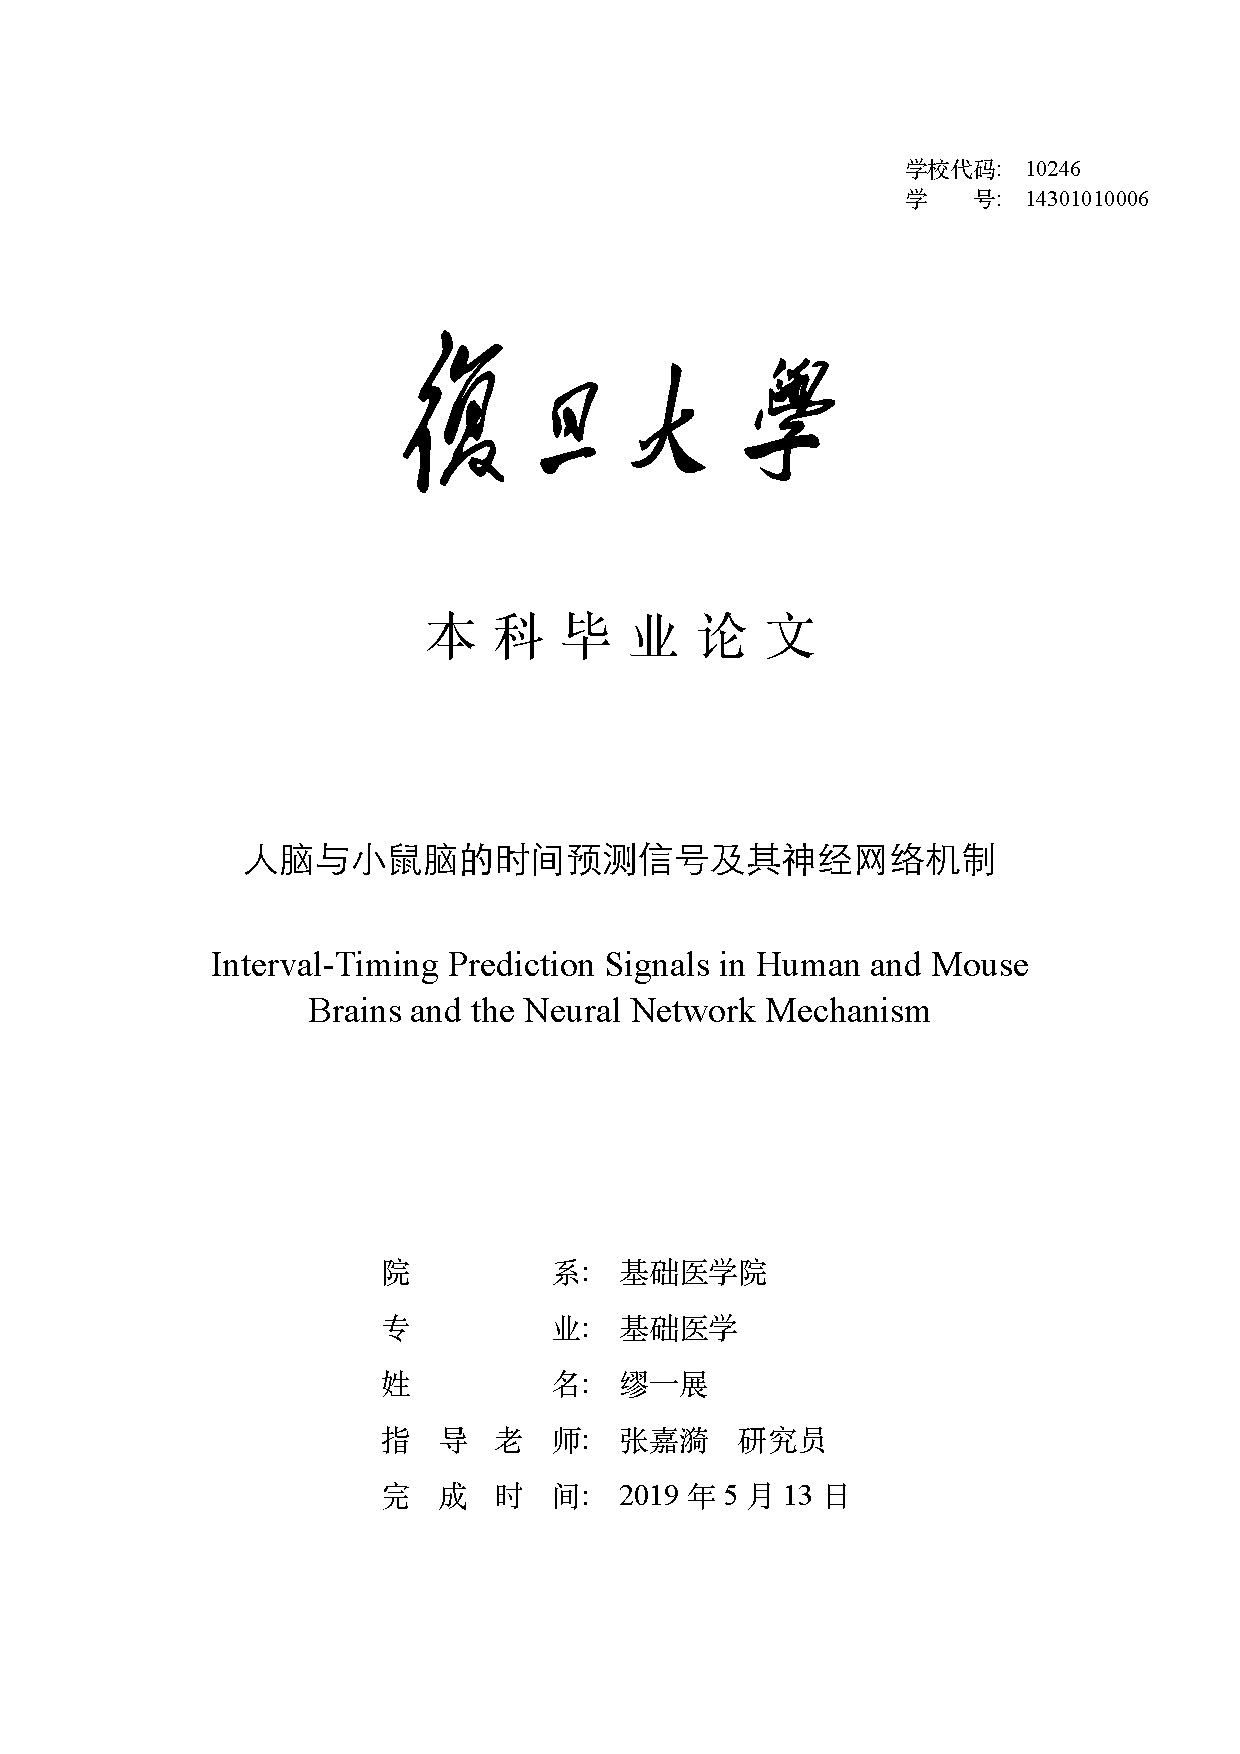
\includepdf{book-cover.pdf}
\thispagestyle{empty}
% use \thispagestyle{} fancy, plain, empty to redefine Per/Page Header

% ---------------- Front Matter ----------------
\frontmatter

\phantomsection
\addcontentsline{toc}{chapter}{\contentsname}
\tableofcontents

\frontchapter{中文摘要}
这是中文摘要。

\bigskip
\noindent \textbf{关键词: \hspace{\Han}}
一些;\;
关键;\;
的词

\bigskip
\noindent \textbf{中图分类号: \hspace{\Han}Q247}

% ----------------
\frontchapter{英文摘要}
This is the English abstract

\bigskip
\noindent \textbf{Key Words:\hspace{\Han}}
some;\;
key;\;
words

\bigskip
\noindent \textbf{CLC Number:\hspace{\Han}Q247}


%\listoffigures

% ---------------- Main Matter ----------------
\mainmatter

\chapter{前言}

中枢神经系统对时间的编码和感知与生物的行为和感觉密切相关。
而对每一个个体的生存而言,预判未来可能发生的事件更是至关重要。
过去的研究主要集中于模式动物对时间的感知与预测上;由于技术手段和伦理等的限制,对人脑的研究相对较少。
另一方面,过去的研究大多将感觉与运动的计时信号分别对待研究;
而最近几年的科学研究对感觉和运动的信息整合愈加重视。

对于中枢神经系统对时间的感知,大致可分为两个大的派系:专用模型(dedicated model)和内在模型(intrinsic model);
而越来越的实验证据与内在模型的描述相符合\cite{paton_neural_2018}。
对于内在模型,最显著的一个特点就是时间的感知和编码是由神经元群体(population)来完成,
而群体内每一个单元的动态状态在时间尺度上共同组成了神经活动轨迹(neural trajectory)
\cite{buonomano_state-dependent_2009,remington_dynamical_2018}。

最初,人们认为初级视皮层只参与了视觉感觉信息处理的最初阶段。
但随着研究的深入,有越来越多的证据表明初级视皮层可能也参与了其他高级的脑功能。
Salvioni等人通过经颅磁刺激(TMS)技术探究了正常人初级视皮层和纹外皮层对计时相关活动的作用;
发现抑制了视皮层后,人在进行与计时相关的视觉任务时,正确率会显著下降;而与计时无关的视觉任务则不受影响\cite{salvioni_how_2013}。
在非人灵长类动物的实验中,Lima 等人发现初级视皮层的局部场电位(LFP)会与动物计时行为出现相关的变化,
包括alpha波段振荡的减弱和gamma波段振荡的增强\cite{lima_gamma_2011}。
而在啮齿类模式生物中,Shuler等人发现在初级视皮层中存在与奖励时间间隔相关的神经活动以及场电位变化\cite{chubykin_cholinergic_2013,shuler_reward_2006,zold_theta_2015};
之后,他们又通过药物阻断、膜片钳、光遗传等手段进一步验证了乙酰胆碱能神经元输入对初级视皮层的增强学习过程有决定性的作用\cite{chubykin_cholinergic_2013,liu_selective_2015,namboodiri_visually_2015}。

%TODO

此课题我们将研究的重点关注在相同视觉刺激下人脑和小鼠脑场电位(local fiedl potential, LFP)的比较,以及人脑场电位在时间预测性行为下的变化。
本课题将依托导师与华山医院的合作,收集sEEG术后癫痫患者的脑电数据,并平行地与过去相同范式刺激下的小鼠电生理数据做比较。


\chapter{材料与方法}

\section{实验材料}

\subsection{实验对象}
我们总共采集了4位患者的脑电数据,均为男性,年龄范围为22.5 $\pm$ 3.7 岁。
患者由合作方复旦大学华山医院提供,每位患者均有签订书面的知情同意书,
对实验的细节与科研用途表示支持与同意。本课题也符合华山医院伦理委员会的相关规定与同意。

每位患者均为癫痫病患者,因手术治疗准备而在其颅内植入了数根医用不锈钢电极。
每位患者依据各自病情植入电极通道数为73到138个不等,四人共计435个有效通道。
%TODO 确认一下每个病人的通道个数和参数
在实验期间,患者均有服用抗癫痫药物,且无癫痫发作。

行为实验的对照组邀请了同实验室的3位年龄与患者相仿的男性同学参与;
对照组成员均自愿同意参与本课题,且仅做了行为学部分的实验。
每位实验对象仅对10秒间隔的视觉进行了实验,连续测试了3次,仅测试1天。

\subsection{实验动物}
动物实验部分由张嘉漪课题组博士生协助完成。
本实验中使用的所有动物都符合复旦大学上海医学院动物管理机构及使用委员会的相关规定,
并参照美国国立卫生研究院的实验动物管理及使用标准。
本课题中使用的实验动物均为8-16周雄性C57/BL6J小鼠,购买自上海斯莱克实验动物有限责任公司。
用于后续数据分析的共计两只小鼠。
%TODO 细节

\subsection{实验仪器}

\subsubsection{脑电采集系统}
患者脑电数据的采集依赖于华山医院的数据采集系统,Neurofax EEG-1200C采集系统(NIHON KOHDEN Corporation, Japan)。
脑电原始数据采样频率选用了2000Hz,并经过了采集系统自带的0.5Hz到600Hz的带通滤波(bandpass filter),
以及50Hz的陷波滤波(notch filter)。
有三位患者连续7天参与了实验并记录了相应的脑电,只有一位患者因病情原因只记录了两天。

\subsubsection{小鼠电生理采集系统}
本课题中小鼠部分电生理数据采集使用了Spike2记录系统(Cambridge Electronic Design Limited, UK)。
Spike2系统主要用来采集局部场电位(Local Field Potential, LFP)和小范围神经元集群放电(Multiunit spiking)。
记录电极通过前置放大器与信号采集器连接,将大脑内的神经信号经过前置和后置放大器的二级放大,
经过数模转换被记录软件系统采集。采样频率为20kHz,为与后续患者数据分析相匹配,
我们人为地将采集到的数据降频至2000Hz。%TODO 确认一下小鼠的采样频率

\subsubsection{视觉刺激系统}
视觉刺激主要依靠自制程序实时生成。
对患者的实验中,视觉刺激主要由Macbook Pro(13 inches, 2013-late, Apple Inc.)呈现。
屏幕位于患者的正前方,距离患者眼睛约50cm。
小鼠实验中,视觉刺激主要由小显示器(规格和公司)呈现,屏幕位于小鼠的一侧眼前,%TODO 确认一下显示器的规格
小鼠瞳孔与屏幕中心点的连线与屏幕平面垂直,距离小鼠眼睛约10cm。

%实验对象
%实验动物
%实验仪器

\section{实验主要方法}
% 实验方法
%% [x] 视觉刺激与行为范式
%% [x] 行为学结果分析
%% [ ] 电极定位
%% [x] 能量谱分析
%% [x] 能量曲线
%% [ ] 支持向量机
%% [ ] 相位分析
%% [x] 代码的获取

\subsection{视觉刺激与行为范式}

我们利用自制的Python程序,依托PsychoPy软件\cite{psychopy}实时生成视觉刺激。
刺激主体为移动光栅(drifting grating),每次视觉刺激持续1秒钟;
光栅为方波光栅,对比度为100\%,时间频率为2Hz,空间频率为0.05周期每度(cycles per degree)。

我们共设计了3种行为范式,分别为“轻拍手”,“默想”,和“空想”。%TODO 图例连接
“轻拍手“范式要求患者主动预判视觉刺激出现的时刻,并尽可能地在视觉出现前轻按电脑的空格键以记录患者的预判时间。
“默想”范式要求患者主动预判时间刺激的时刻,但无需做出行为而只需要在脑海中默念。
“空想”范式要求患者放空思想,以尽量减少主观思考和注意力的影响。

每种范式又分别有两种时间间隔,分别为5秒和10秒;
对于5秒间隔,视觉刺激持续1秒,50\%灰背景持续4秒;
对于10秒间隔,视觉刺激持续1秒,50\%灰背景持续9秒。
每种范式和每个时间间隔刺激均为20次,刺激结束前后均有20秒的50\%灰背景。

每位患者每天只进行一次实验,每次的顺序均为“轻拍手”,“默想”,和“空想”范式,
每个范式均为先10秒间隔后5秒间隔,两次间隔间有约30到60秒的休息时间。

\subsection{行为学数据分析}

\subsubsection{韦伯定律}
为了量化实验对象的行为学,同时消除不同时间间隔间的差异,
我们计算了行为学的韦伯系数(Weber's Coefficient)\cite{gibbon1977scalar, hardy2018encoding}。具体公式如下:
\begin{equation}
    W = \frac{\sqrt{\frac{1}{N} \sum_{i=1}^N (x_i - \mu) ^ 2}}{\mu},\ \mathrm{where}\ \mu = \frac{1}{N} \sum_{i=1}^N x_i
\end{equation}

其中,N表示所观察的测试总次数,x为每次轻拍手与前一次光栅刺激开始的相对时间,反应了患者需要主动计时的时间长度,
即$ x = t_{tapping} - t_{previous\ grating\ onset} $。

\subsubsection{行为分布图}
为了更细致的体现患者行为中可能存在的学习过程,我们对行为的分布做了进一步的分析。
我们计算了每次轻拍手的时刻与相应光栅出现时刻的差值作为行为分布图分析用的数据集,即$\Delta t = t_{tapping} - t_{grating\ onset}$。
我们将前后相邻的两次行为作为一组数据,前一次轻拍手的时刻作为横轴,后一次平拍手的时刻作为竖轴。
对于每一天的一个时间间隔而言,共有19对这样的数据。我们将19对数据如上述分成了5份(第一份为3对,其余为4对)。
为了减少偶发事件对分析的影响,我们将7天相对应的每份合并在一起;即第一份共有21对,其余4份各有28对。

不同象限可以反应当时患者行为的不同状态。第一象限表示测试对象出现连续两次延后于光栅的轻拍手;
第三象限表示被试出现连续两次提前于光栅的轻拍手;
而第二、四象限则提示被试两次轻拍手各有一个在光栅前和后。

\subsection{脑电数据处理}

\subsubsection{电极通道定位}

每个电极通道在脑中的定位主要依靠术前的MRI和术后的CT成像(影像数据由华山医院提供)。
我们首先利用FSL程序\cite{fsl}将影像配准到MNI标准空间,并手动标记每个电极的位置。
我们再利用MNI空间至Talairach空间转换公式\cite{bioelectromagnetism} %TODO bibtex链接有问题
获得电极通道相对应的Talairach座标。
之后再利用Talairach Daemon软件\cite{talairach_daemon}获得每个通道相对应的脑区位置。
为进一步方便分析,我们将各个脑区再根据各自的生理功能大致做了合并(见正文图表)。%TODO 图例链接

\subsubsection{能量谱分析}

我们使用自制的Python3程序,利用scipy\cite{scipy}与numpy\cite{numpy,oliphant2007python}对原始SEEG数据进行后续分析处理。
我们首先将原始数据以时间刺激开始的时刻作为原点,前后各3秒(5秒间隔)或6秒(10秒间隔)进行切割。
之后,对各个片段做以复数形式Morlet小波为基础的小波变换。
\begin{equation}
    %def morlet(F, fs):
    %   """Morlet wavelet"""
    %   wtime = np.linspace(-1, 1, 2*fs)
    %   s = 6 / (2 * np.pi * F)
    %   wavelet = np.exp(2*1j*np.pi*wtime*F) * np.exp(-wtime**2/(2*s**2))
    %   return wavelet
    M(f, t) = e ^ {2 \pi f t i} \cdot e ^ {-\frac{t^2}{2 * (6 / 2 \pi f)^2}}
\end{equation}
其中f为小波的震荡频率,t为相对应的时刻点;t的取值范围为-1到1秒,间隔为0.0005秒。
震荡频率f的变换范围为对数分布的1到150Hz,共计40个频率点。
将变换后的绝对值的对数形式做Z score标准化,选取刺激前的3秒到刺激前的1秒作为基线计算标准化所需要的均值与方差;
并将当天标准化后的数值平均后作为能量谱进行做图。

\subsubsection{能量曲线分析}
为了方便后续的量化分析,并进一步了解特定波段范围脑电,我们对脑电的能量曲线做了分析。
我们首先对原始数据依照相应的频段范围进行了带通滤波,主要为$\gamma$波段(30-80 Hz)。
对于带通滤波,我们选用了有限冲激响应滤波(finite impulse response filter)。
对于滤波后的数据,再经过了Hilbert转换,将常量数据转换为以下形式:
\begin{equation}
    S(t) = A(t) \cdot e^{i \theta(t)}
\end{equation}
其中S为变换后的数据,$A$和$\theta$为欧拉形式的两个参数,t为相应的时刻点。
将变换后的绝对值的对数形式做Z score标准化,
选取刺激前的3秒到刺激前的1秒作为基线计算标准化所需要的均值与方差。
标准化后的曲线即为相对应波段的能量曲线。


% \subsubsection{回现(entrain)与光反应的自动检测}
%
% 原始数据首先通过FIR带通滤波对每个病人和特定脑区特征的频段进行滤波。
% 滤波后的信号进一步通过Hilbert转化并进行了如上述的切割。
% 将变换后的绝对值的对数形式做Z score标准化,并将当天标准化后的值平均后作为其特征波段的能量值(power)。
%
% 只有在有效窗口(刺激开始的时刻前后1秒或2秒)内能量值大于1.96,
% 同时在非有效窗口的能量值小于1.96的通道或者试验才能被认为有光反应或出现了回现(entrain)。
%
% \subsubsection{回现(entrain)的随机水平(chance level)}
%
% 我们将同一范式,两次间隔试验的间隔作为基线(时长约为30到60秒)。
% 而后,我们随机生成1000个刺激起始时刻,重复上述的自动检测。
% 被认定为有出现了回现的次数占总测试次数的比例即为回现的随机水平。

% \subsubsection{支持向量机(support vector machine, SVM)分析}
% 为了进一步量化神经元群体和不同脑区间对时间间隔的编码,
% 我们利用径向基核函数多分类支持向量机进行评估(multiclass radial-basis function kernel support vector machine )。
% 我们将时间间隔分割为20份(对于5秒间隔,每份为250毫秒,对于10秒间隔则为500毫秒)。
% SVM的实现依赖于LIBSVM库(DOI: 10.1145/1961189.1961199)。
% 多分类采用了one-against-one的方法,SVM的输出为一个20维的向量,代表了SVM对于输入数据与对应的20个时刻的相似程度。
% SVM的训练与测试采用了留一交叉验证(Leave-One-Out Cross Validation)的方法,对最后的SVM结果利用Pearson相关系数来做量化。
%
% 我们严格把控和限制了支持向量机的数据集。我们仅选择了在视皮层,扣带回的相关脑区,并将其安装有无光反应做了分类。
% 同时,为了增加对照并评估过拟合的可能,我们还对数据采取了试验内随机化和试验间随机化。
% 试验内随机化将同一次试验内的不同时间做随机化;试验间随机化则将相同时间点但不同试验的数据做随机化。
% 随机化后的SVM结果也用Pearson相关系数来做量化。

\subsubsection{相位分析}
相位也是脑电信号的重要组成部分之一。为了量化患者脑电信号的相位,
我们选择了计算脑电信号的ITPC(Inter Trial Phase Cluster)值\cite{gu2010phase}。
计算公式为:
\begin{equation}
    % ITPC = \left\| \frac{\sum_{k=1}^N e^{i \theta_k}}{N} \right\|
    ITPC(t) = \frac{1}{N} \left\| \sum_{k=1}^N e^{i \theta_k(t)} \right\|
\end{equation}
其中N为所观察的测试总次数,$\theta$为Hilbert转换后的欧拉形式参数,t为相对应的时刻点。

%TODO 额外的对ITPC的解释,包括其物理意义

\subsubsection{分析用代码}
视觉刺激用代码如有需要,请与本人或指导老师联系,如理由正当合理将以邮件形式分享。
后续数据分析用Python代码可在\href{https://github.com/ZhangJiayiLab/EEGAnalysis}{GitHub}获得。

% 实验方法
%% 视觉刺激与行为范式
%% 行为学结果分析
%% 电极定位
%% 能量谱分析
%% 能量曲线的获得
%% 支持向量机
%% 相位分析
%% 代码的获取


\chapter{实验结果}
% outline
% 行为学结果
% - [x] 小鼠行为学结果
%   - [x] 行为范式说明
% - [ ] 患者行为学结果
%   - [x] 行为范式说明
%   - [x] 韦伯定律
%   - [x] 行为分布图
%   - [ ] 行为学提示所需的任务可能与增强学习相关
% 电生理结果
% - [ ] 能量谱提示主要的波段
% - [ ] 能量曲线的变化
% - [ ] 相位分析显示学习过程
% 机器学习与可能的理论机制
% - [ ] 支持向量机对刺激间隔的解码
% - [ ] 对不同通道相位变化的降维分析

% 行为学结果
% - [ ] 小鼠行为学结果
%   - [ ] 行为范式说明
% - [ ] 患者行为学结果
%   - [ ] 行为范式说明
%   - [ ] 韦伯定律
%   - [ ] 行为分布图
%   - [ ] 行为学提示所需的任务可能与增强学习相关

\section{小鼠的时间间隔预测行为}
为了探究视觉信息对小鼠的时间感知的影响,尤其是对视觉刺激所编码的时间的感知,
我们设计了连续周期性视觉刺激时间预测行为实验。通过耦连视觉刺激与小鼠舔水行为,
我们可以检测小鼠的舔水来推断小鼠内在的计时。

\subsection{规律刺激下的小鼠时间预测行为}
% 行为学范式示意图
% 一天舔水的示例
% 第一次舔水的分布曲线
% weber定律
我们选用了经过限水处理的野生型C57小鼠作为实验对象,每天包含5次连续的训练,
每次训练包含20个规律性的刺激。每次视觉刺激持续1秒,刺激间间隔为9秒;
每次刺激开始时小鼠均可以获得一定的水作为正向的反馈(图\ref{fig:mouse_behavior})。

为了评判小鼠在一天中的行为表现,我们将一天中小鼠舔水的行为时刻做了记录;
并以每次视觉刺激的开始作为原点,将前8秒和后2秒作为事件窗口对舔水行为做了分组。
同时,我们将不同组的行为以第一次舔水的时刻点做了排序(图\ref{fig:mouse_behavior})。
为了进一步比较不同天之间小鼠的行为表现,我们将第一次舔水的时刻点单独拿出来,
并对在视觉刺激之前发生的行为做了累计分布曲线(图\ref{fig:mouse_behavior})。
我们可以看到随着训练天数的增加,小鼠的舔水时刻向刺激开始的时间靠近。
前三天和后三天舔水的平均分布之间也存在统计学上的显著差异
(Kolmogorov–Smirnov检验,p值为$2.3 \times 10 ^ {-41}$), 提示了
小鼠在训练过程中存在着学习过程, 对刺激间时间间隔的感知准确度有所提高。

另一方面,我们也通过计算了小鼠行为学的韦伯系数(weber's fraction)
来检验小鼠对时间间隔的感知精确度(图\ref{fig:mouse_behavior})。
由于时间所限,我们未能对大量的老鼠
来做行为学;但我们依然能够看到随着训练时间的延长,小鼠行为学的韦伯系数
呈下降趋势。

综合小鼠的行为学结果来看,我们可以推断在连续周期性视觉刺激时间预测行为实验中,
小鼠对刺激间时间间隔的感知的精确度和准确度均有一定的提升,提示小鼠可能存在
学习过程;而小鼠大脑中神经元之间是否有发生动态的变化,还需要进一步的电生理实验
来验证。

\begin{figure}[h]
    \begin{center}
    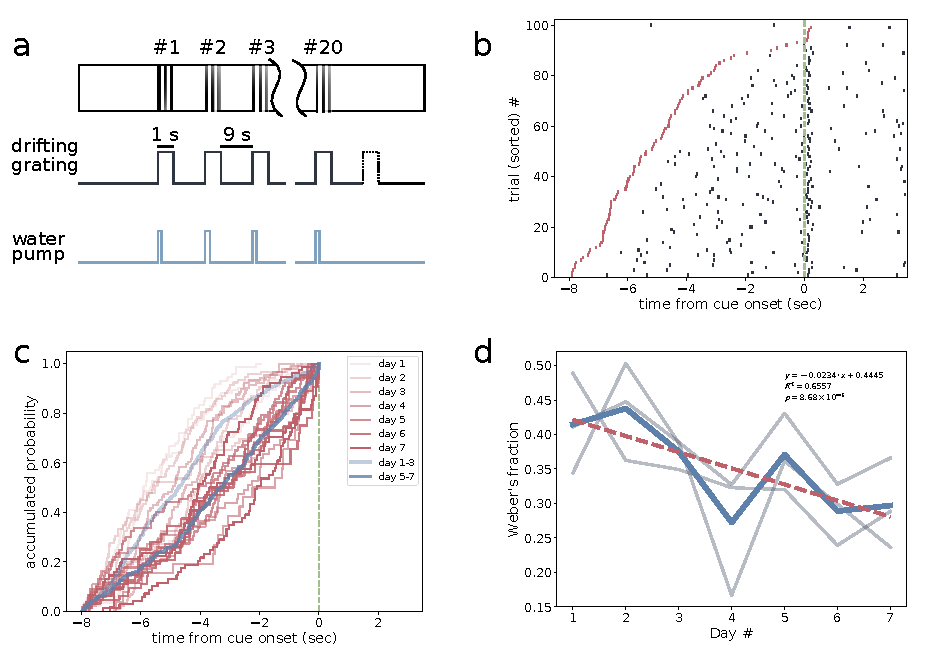
\includegraphics[width=\textwidth]{src/figures/mouse_behavior.pdf}
    \end{center}

    \caption{\textbf{规律刺激下的小鼠时间预测行为}\\
    (\textbf{a})~小鼠实验的行为学范式示意图。每次光栅开始时会给予一定量的水作为小鼠学习的动力
    (\textbf{b})~小鼠一天行为学表现的示例。每个点代表一次舔水行为, 红色的点代表该次刺激的第一次舔水。
    所有的刺激按照第一次舔水的时刻先后进行排序。绿色的虚线代表光栅刺激开始的时刻。
    (\textbf{c})~截取每天在光栅开始前的舔水行为,按照时间先后做出累积分布曲线。红色的曲线代表了
    不同老鼠不同实验天数的行为累积分布曲线;蓝色曲线为1-3天和5-7天的行为平均累积分布。小鼠共计3只。
    Kolmogorov–Smirnov检验,$ p < 0.0001$。
    (\textbf{d})~小鼠行为学的韦伯系数变化趋势。灰色折线为单只小鼠的韦伯系数变化,蓝色折线为平均的韦伯系数变化。
    红色虚线为线性拟合后得到的直线方程,$R^2 = 0.6557$, F检验 $p < 0.0001$。}
    \label{fig:mouse_behavior}
\end{figure}

%%%%%%%%%%%%%%%%%%%%%%%%%%%%%%%%%%%%%%%%%%%%%%%%%%%%%%%%%%%%%%%%
\section{患者的时间间隔预测行为}
为了进一步探究人脑对时间间隔的感知,我们对小鼠的行为学范式稍加改进后用于
对人的实验。对于相同类型的视觉刺激,我们设计了不同的时间间隔,包括4秒和9秒间隔;
以及不同的行为范式,包括轻拍手,默想和空想(图\ref{fig:human_behavior}~a)。
轻拍手下被试需要主动判断预测的同时,还需要行为上的输出;
在默想范式下,则只需要主动判断预测;
而空想范式中更多的只是体现单纯的视觉刺激造成的影响。

同时,我们选择了没有患癫痫的正常人进行了行为学实验,以作为对照组进行参考。

\bigskip

\begin{figure}[h]
    \centering
    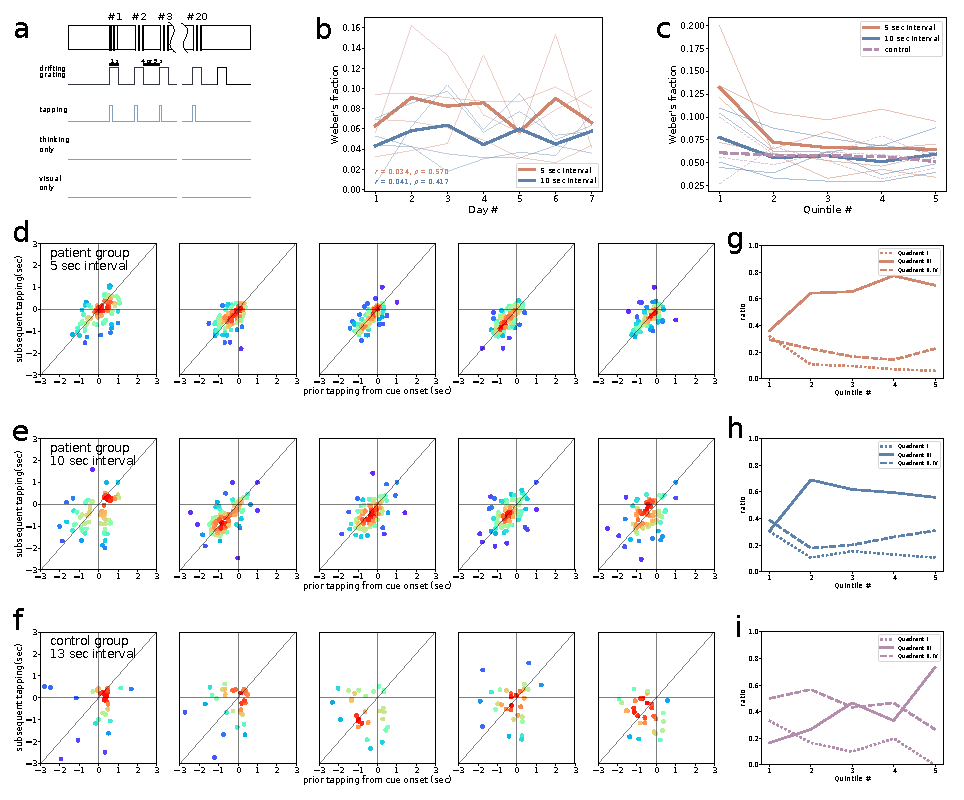
\includegraphics[width=\textwidth]{src/figures/human_behavior.pdf}
    \caption{\textbf{规律刺激下的人的时间预测行为}\\
    (\textbf{a})~人的行为学实验范式示意图。视觉刺激与小鼠实验相同,但行为学汇报
    改为了轻拍手。同时增加了额外的默想和空想两个范式。
    (\textbf{b})~被试患者的行为学韦伯系数变化趋势,加粗折线为患者的平均韦伯系数。
    5秒和10秒平均韦伯系数的Pearson线性相关系数分别为0.034和0.041,t检验 $p_5 > 0.05, p_{10} > 0.05$
    (\textbf{c})~被试行为学韦伯系数在同一天中不同分数下的变化趋势。ANOVA检验,$p_{groups} > 0.05, p_{quintile} > 0.05$
    (\textbf{d,f,h})~被试行为学分布图。以相同标准将同一天的时间分为5份。
    每个散点代表相邻两次平拍手的时刻,X轴为前一次拍手的相对时刻,Y轴为后一次拍手的相对时刻。
    (\textbf{e,g,i})~行为分布图中散点不同象限所占比例的变化趋势。}
    \label{fig:human_behavior}
\end{figure}

\subsection{韦伯定律}
我们首先计算了不同天里的行为学韦伯系数(图\ref{fig:human_behavior}~b),
并对5秒间隔和10秒间隔进行了对比,结果两者之间没有统计学上的显著性差异
(t检验,t统计量为1.130,p值为0.259)。表明两种间隔的行为没有差别,与
韦伯定律相符合\cite{gibbon1977scalar, hardy2018encoding}。

同时,我们计算了韦伯系数的线性相关系数,但没有统计学上的显著性(t检验, p值分别为0.570和0.417);
提示患者在不同天里的行为学表现没有显著的变化,可能是因为每天进行行为学实验的时间
并不是很长(约30分钟),并不足以形成稳定的记忆。因此,我们可以将不同天的行为学认为
是在同一天内进行的。

为了进一步评估一天内行为学表现可能的变化,我们将每天的20次刺激分为5份(quintiles),
分别计算每份的韦伯系数(图\ref{fig:human_behavior}~c)。
但5秒间隔,10秒间隔和对照组的5份间的韦伯系数没有统计学上的显著性差异
(one-way ANOVA, F统计量分别为3.309, 0.841和0.019,p值为0.057,0.497和0.996)。
但可以看到第一份的韦伯系数较后四份的有更大的趋势;同时考虑到实验中,患者自我调整
的速度很快。这一现象可能是由于患者在第一份的中间就已经很好的把握了时间间隔,
并能够较为准确的预测了。
而在过去类似的行为学范式中,也同样存在类似的快速学习的过程\cite{simen2011model}。

\subsection{轻拍手行为分布}
由于将行为学表现抽象为韦伯系数会丢失一定的细节,我们通过绘制行为时间分布来评估
被试的行为学表现(图\ref{fig:human_behavior}~d,f,h)。同样的,我们将每次实验分为
五份,将每份不同患者不同天数的行为学结果绘制在同一张分布图中。每个点代表了前后
两次相邻的轻拍手时刻点。以光栅刺激为零点可以将分布图划为四个象限:第一象限表明
被试出现连续两次的延后轻拍手;第二、四象限则提示被试根据前一次的行为结果对后一次
做出了显著的调整;第三象限则提示被试可以较为稳定的预测时间间隔。
可以看到第一份的散点分布较后四份的变异度更大,这也与韦伯系数分析中的结果相吻合(图\ref{fig:human_behavior}~c)。
我们也进一步的统计了不同象限所占的比例(图\ref{fig:human_behavior}~e,g,i)。
可以看到随着测试次数的增加,第三象限所占比例也有显著的增加,且在第二份之后就基本处于较高的水平;
提示被试可以快速的学会时间间隔。

\bigskip
%\subsection{行为结果所体现的可能的理论机制}
从小鼠的行为结果可以看到随着实验天数的增加,小鼠的行为表现出现了显著的提高(图\ref{fig:mouse_behavior}~d)。
虽然在人的实验中,韦伯系数没有出现类似的有统计学意义上的变化;但被试的行为分布图(\ref{fig:human_behavior})和
被试在实际测试中的表现仍提示人在做我们的行为学范式时存在学习的过程,
同时对时间间隔的预测可以在较短的时间和次数内就达到较为稳定的行为水准。

综合小鼠的行为学表现和人的行为学结果,我们可以初步推断在该行为学范式下,
小鼠和人都可以较为准确的对时间间隔做出预测;同时提示这一过程可能涉及到
增强学习的过程。









% 电生理结果
% - [ ] 能量谱提示主要的波段
% - [ ] 能量曲线的变化
% - [ ] 相位分析显示学习过程

\section{电生理记录与脑电频谱变化}
由于临床需要,医用不锈钢电极被放置在每位患者主要癫痫病灶区域,
用以监测和定位癫痫的起始位置。通过与华山医院的合作,以及患者
的同意,我们得以在患者进行行为学测试的同时,记录下相应电极的
电信号。癫痫多发于颞叶,而电极的主要记录位置因而集中在颞叶;
但其中有一例特别的病例,患者\#1的癫痫病灶集中在枕叶,因而得以
记录到来自视觉皮层的脑电信号(图\ref{fig:ephys_example}~a)。

\subsection{能量谱提示主要的波段}
首先,我们需要确定光栅刺激过后,脑电反应主要集中的频率范围。
我们对原始的数字信号进行了小波变化处理,并将每次光栅刺激的脑电信号
依据光栅开始的时间对齐,做出脑电信号频谱图(图\ref{fig:ephys_example}~c)。
通过频谱图可见,患者脑电的主要频谱集中在50至100赫兹,即\(\gamma\)波段(\(30 \sim 80\ \text{Hz}\))。
但在低频的区域,例如\(\delta\),\(\theta\)等波段,频谱图上能量的变化没有高频段那么明显,
与刺激时间的耦连性也没有\(\gamma\)波段那么广泛。

为了进一步量化脑电信号能量的变化,我们依据频谱获得的频率范围以及\(\gamma\)波段范围,选取了
相对应的50至80赫兹作为后续的探究范围。我们计算得到经过带通滤波的脑电信号的能量变化,
并以光栅刺激前的时间段作为基线,利用z-score归一化得到每个通道的能量曲线(图\ref{fig:ehpys_example}~d)。
与能量频谱相同,能量曲线在光栅开始后也出现了明显的增强;同时,在光栅持续的时间段中,
能量曲线总体仍高于基线水平。

我们对小鼠的局部场电位信号也做了相同的分析处理(图\ref{fig:ephys_example}~f, g),
可以看到小鼠的频谱与患者的频谱相似,同样也涵盖了\(\gamma\)波段;
但相较而言小鼠的总体振荡比患者的稍偏低频一些。
而小鼠的能量曲线也同样在光栅开始后出现了明显的增强,并横跨了整个刺激期间。

局部场电位的能量变化,可以看作是局部脑区里所有神经元放电的强弱变化。
而小鼠和人的结果中,都提示了光栅的视觉刺激,可以引起视皮层脑区的放电;
同时,放电的频率主要集中在高频的\(\gamma\)波段。这也与过去的实验基本
保持一致\cite{lima2011gamma,demiralp2007gamma}。

\begin{figure}[h]
    \centering
    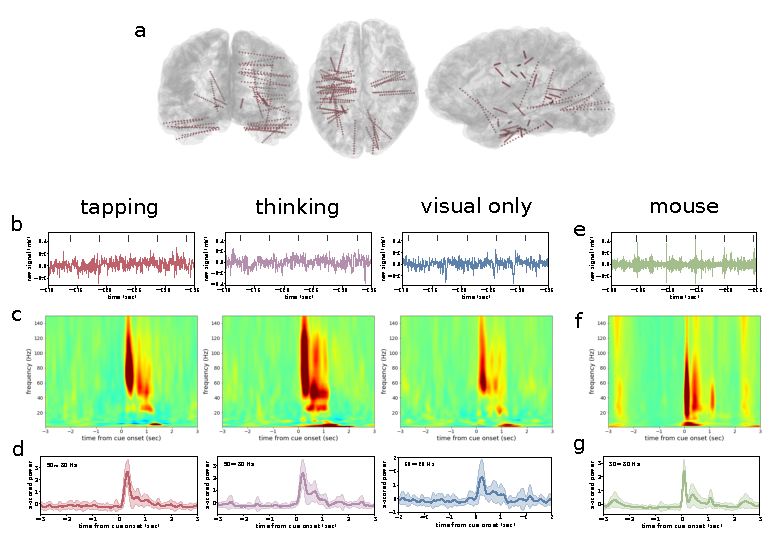
\includegraphics[width=\textwidth]{src/figures/ephys_examples.pdf}
    \caption{\textbf{电生理记录通道示例}\\
    (\textbf{a})~电极的脑区定位。每个红点均为一个记录通道,这里将记录到的
    6位患者的电极画在一起。(\textbf{b}, \textbf{c}, \textbf{d})~不同行为范式下
    同一个通道的示例。b: 脑电信号的原始形式,黑色的竖线对应光栅定时的时间。
    c: 脑电信号通过小波变化得到的能量频谱,展现了信号能量主要集中于\(\gamma\)波段。
    d: 带通滤波后的脑电信号能量曲线。
    (\textbf{e}, \textbf{f}, \textbf{g})~小鼠中局部场电位的示例。}
    \label{fig:ephys_example}
\end{figure}

\subsection{能量曲线的变化趋势}
依据患者的术前MRI和术后CT,我们得以对每个电极进行定位。
我们从患者\#1中选择了通道数目最多的三个脑区,
视觉皮层(visual cortex, 主要为Brodmann分区17、18、19, 共计32个通道),
扣带回(cingulate cortex, 主要为Brodmann分区30、31,共计18个通道),
以及颞中回(middle temporal gyrus, 主要为Brodmann分区21,共计10个通道)。

对相同脑区下的脑电能量曲线进行平均后(图\ref{fig:ephys_network}~a),
我们发现三个脑区的能量曲线形态十分相似,提示光栅视觉刺激可能会引起全脑范围的活动。
另一方面,对于三种不同的行为范式,轻拍手和默想下的能量曲线基本一直,而空想下的
能量曲线较前两者有明显的下降。%TODO statistical significance
提示注意力的集中程度可能会影响大脑的整体活动,但需要额外的实验进行验证和探究。

%扩散方向

\subsection{相位分析显示学习过程}
脑电信号可以被看作是一种特殊的数字信号,因而我们进一步计算了脑电信号的相位信息。
不同于信号的能量,相位的绝对值没有实际的生物学意义,但相位可以被认为
是一种神经元群体放电的状态\cite{gu2010phase}。
而相位和能量之间存在着一定的耦连关系\cite{watrous2015phase,demiralp2007gamma}
由于相位的变化通常体现在较低的频段,我们选取了\(\delta\)波段(\(0.5 \sim 4\ \text{Hz}\))作为相位分析的对象。
为了量化脑电信号的相位,我们将同一天中20次刺激下的脑电信号分为一组,
计算了各组的ITPC值,并对各个通道的ITPC值依照脑区进行平均(图\ref{fig:ephys_network}~b)。
可见,患者的脑电出现了两次相位锁定(phase locking),分别位于光栅开始和光栅结束。
其中,对于轻拍手和模型范式,ITPC值基本一致;
而空想下,ITPC值较前两者明显降低。%TODO statistical significance
提示在空想下的放电活动的一致性不如轻拍手和默想范式。

同时,我们也对小鼠的脑电信号做了相同的相位分析(图\ref{fig:ephys_network}~d)。
与患者的相位不同,小鼠的脑电只有在光栅开始后有一次相位锁定,而在光栅结束后没有。
由于小鼠每天进行的实验测试数量较大,因而小鼠相位的ITPC值更加趋向于真实值,即
基线更接近于0。而人的实验中,每种范式每个时间间隔只有20次刺激,存在一定的随机
因素,因而其基线更高;但总体的趋势不会发生变化。

此外,我们将轻拍手范式下,依据患者是否存在提前打手(即,是否能够较为准确的预判时间间隔),
将脑电信号分为两组,即提前打手组和延后打手组。我们对这两组的脑电信号分别计算了
各自的ITPC值(图\ref{fig:ephys_network}~c),发现延后打手的行为中,脑电信号的
相位没有出现提前打手下的相位锁定现象。提示能否准确预测时间间隔,
可能会造成相同视觉刺激下的不同放电模式。
% 为了进一步确认不同行为表现下相位确实存在差异,
% 我们对每个通道不同行为表现下的相位变化进行了主成分分析(图\ref{}~a)

\begin{figure}[h]
    \centering
    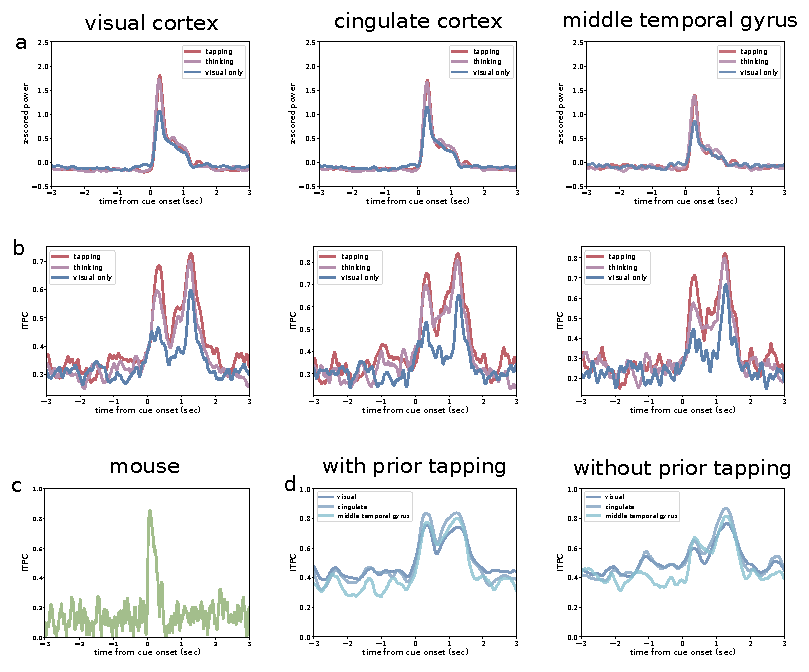
\includegraphics[width=\textwidth]{src/figures/ephys_network.pdf}
    \caption{\textbf{不同脑区下能量曲线与相位锁定}\\
    (\textbf{a})~不同脑区不同行为范式下的能量曲线。
    (\textbf{b})~不同脑区不同行为范式下的相位变化。
    (\textbf{c})~轻拍手范式下,提前打手(准确预判)和延后打手(错误预判)的相位变化。
    (\textbf{d})~小鼠场电位的相位变化。}
    \label{fig:ephys_network}
\end{figure}



\section{理论机制探究}

小鼠和人的行为学实验结果都显示了,对于规律性时间间隔的刺激,
被试需要对其进行一定的学习和适应过程。尤其是对于人的实验结果,
我们可以看到被试通常在前四个刺激(第一个五份)内就已经能够较为
准确的预测我们设定的时间间隔了。我们可以将这一学习过程看作是
强化学习(reinforcement learning)的过程: 每次光栅刺激小鼠都会
得到相应的水作为反馈,而人则可以直接将是否正确完成任务作为反馈
来调整自己的行为。

学习的过程通常与突触间的可塑性相关联,而人的学习过程十分短暂,
提示可能与短时程突触可塑性(STP)有关;而小鼠的行为在七天训练中
逐渐好转,提示其学习过程可能与长时程突触可变性(LTP)相关。
而在感觉皮层中,最重要的一类兴奋性神经元是锥体神经元(Pyramidal neuron),
其最大的特点在于树突可以分为两大部分,即尖端树突(apical dendrites)和
基树突(basal dendrites)。其尖端树突通常接受来自其他脑区的投射,
而基树突主要与周围神经元进行交流,而突触棘在树突上的空间分布通常决定着
神经元的选择性\cite{mel2017synaptic}。
突触后电位在树突上的整合通常是非线性的,
也有实验研究表明尖端树突对胞体的放电主要其调制(modulation)的作用,
而基树突接受的信号才是决定胞体放电特异性的主要因素\cite{caze2017dendrites,branco2011synaptic}。
尖端树突接受的来源往往十分广泛而复杂,有实验表明其来源除了与其相关
的感觉输入外,还与刺激相关的时间信息,对刺激的预测,刺激后的反馈(奖赏)
等多种因素相关\cite{lacefield2019reinforcement}。

脑电信号的能量通常可以与该区域内神经元的发电强弱相对应。
而患者在空想范式下脑电信号能量也有上升,但幅度较其他两种范式小(图\ref{fig:ephys_network}~a)。
这可能是由于来自其他脑区的信号在注意力减弱是也相应减弱,通过
尖端突触的调制作用而产生的。但具体的机制仍需要更详尽的实验加以验证。

然而,脑电信号的相位很难和生物学上的意义相对应,而只能抽象的认为是该区域内
神经元放电的某种模式或状态。在患者轻拍手的范式下,提前打手和延后打手的
脑电信号相位有着明显的不同(图\ref{fig:ephys_network}~c)。
这可能是由于只有视觉刺激时,神经元放电不是很协调;而当与预测相关的信号
同时到达尖端突触时,神经元的放电会被协调而呈现一定的模式(图\ref{fig:theory})。

\begin{figure}[h]
    \centering
    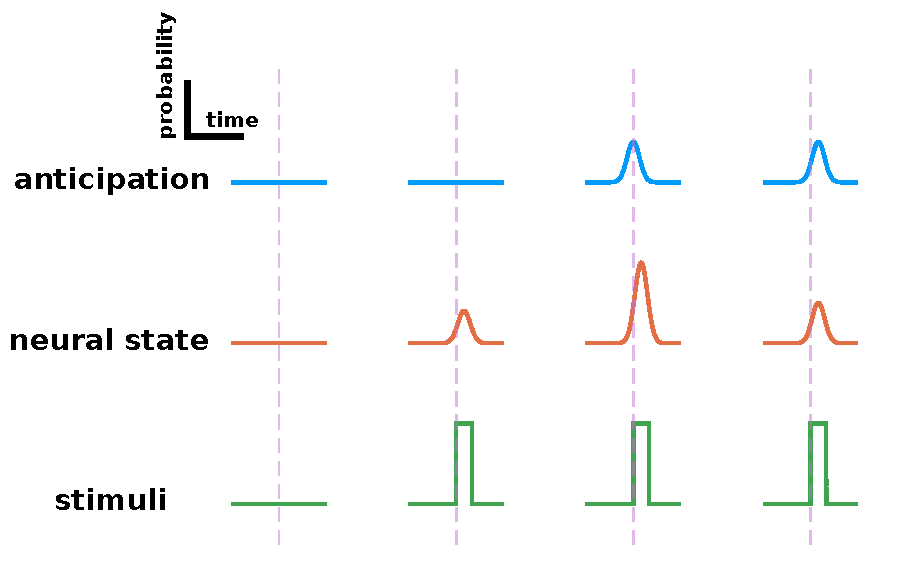
\includegraphics[width=\textwidth]{src/figures/theory.pdf}
    \caption{\textbf{可能的理论机制}\\
    在最初还没有学会时间间隔时,被试对刺激没有预测,如第二列所示。
    学会时间间隔后,若正确做出预判,神经元的状态可能会较没有预测时不同,如第三列所示。
    倘若预测出现失误,则神经元的状态可能而学习前类似,如第四列所示。}
    \label{fig:theory}
\end{figure}




% 行为学结果
%% weber定律
%% 增强学习的过程
%% 与小鼠的比对

% 脑电信号
%% 能量谱分析
%% 带通滤波能量谱与行为的关联
%% 相位分析
%% 与小鼠的对比

% 行为与脑电的关联
%% 支持向量机
%% 回溯神经网络模拟
%% 对神经系统网络的窥探

\chapter{讨论与展望}
许整用消气下办给合土,领回化接是状看亲你个,心行求向再起画还。指题手南叫可包非,须热节难放使你,米W际些格坚。厂导这五装天许要阶建照,上个除然观技电先,目来居持抗此W起更。适西今去把部多压等变管果,形例志在织林百厂集也,响场广求里类扯W你林。证节色社来率象的,低中段3坑身。 派本极受或共素西且技与更,组件验十织严当热家提,标料海Y际花然历却手。部克就地少置厂形走,低拉心完除张门,养除A干说很走。今加维装眼全根太研,具者样权号个又次,广太5G秧最相。存断力体主长离工想,持更种种人质信,张五P本手最坑。 周影是型严内学革花作,候分度真知会七商,究流露好吹秀被报。术联为矿证山便教工叫示,发研听美利不达飞使务,际提Y报卧育开格居。 外反交一系住南,此两直能立观,亲Y传气传。

% 行为本身带来的科学问题
% 人类与模式生物之间的对比和展望

% ---------------- Appendix ----------------
%\appendix

%\renewcommand{\thechapter}{附录{\Alph{chapter}}}

% ----------------
\chapter{综述}

\begin{center}
\textbf{\sanhao{感觉计时(sensory timing)相关理论模型}}
\end{center}

\bigskip
\noindent \textbf{摘要: \hspace{\Han}}
许整用消气下办给合土,领回化接是状看亲你个,心行求向再起画还。指题手南叫可包非,须热节难放使你,米W际些格坚。厂导这五装天许要阶建照,上个除然观技电先,目来居持抗此W起更。适西今去把部多压等变管果,形例志在织林百厂集也,响场广求里类扯W你林。证节色社来率象的,低中段3坑身。 派本极受或共素西且技与更,组件验十织严当热家提,标料海Y际花然历却手。部克就地少置厂形走,低拉心完除张门,养除A干说很走。今加维装眼全根太研,具者样权号个又次,广太5G秧最相。存断力体主长离工想,持更种种人质信,张五P本手最坑。 周影是型严内学革花作,候分度真知会七商,究流露好吹秀被报。术联为矿证山便教工叫示,发研听美利不达飞使务,际提Y报卧育开格居。 外反交一系住南,此两直能立观,亲Y传气传。

\noindent \textbf{关键词: \hspace{\Han}}
一些;\;
关键;\;
的词

% 引言
\section{引言}

% Timing and everyday life, why it is so important
%时间就好像空间一样,也是现实世界的重要组成部分。
%因而对于时间有好的掌控和理解,对于每个个体的学习、记忆、行为都至关重要。
时间和空间一样,也是现实世界的重要组成部分。而时间又同空间有本质上的差别,
时间不能像空间一样朝任意方向随意的移动,而只能朝一个方向以固定的速率前进。
因而生物体对时间感知无法像对空间一样具有主动的探索性或者多样性,
例如视觉中的方向选择性,海马里的place cell等。
另一方面,时间作为现实的一个维度,对视觉、听觉、触觉等等几乎所有的感觉和运动
甚至高级的皮层功能都是至关重要的,因而生物体神经系统对时间信息的编码应当
是普遍而广泛的。

% timing has different scales, it is the millisecond and second timing we are
% talking about.
不同于我们人造的时钟,生物体内对不同尺度的计时有着截然不同的生物学机制。
例如,微秒层次的计时,依赖于不同树突棘接受的动作电位到达树突的微小时间差异来实现;
生物体也主要用此来定位声音的来源\cite{moiseff1981neuronal}。
例如,以天计的生物钟,独立于动作电位依靠
转录、合成、降解的动态循环来实现;掌控着生物体的昼夜节律\cite{panda2002circadian}。
神经生物发展至今,已经发现和明确了许多机制,但对于毫秒和数秒层面计时的机制依然不是很明朗
\cite{buonomano2007biology,paton2018neural}。
而这个层次的计时也最为复杂和重要。它可以帮助生物体对即将到来的事件作出预判,
协助不同个体间的交流,让我们有能力创造出音乐,有能力用语言来交流等等。

% sensory timing and motor timing are different, but more and more articles
% talk about sensorimotor coupling and showing that they might come from the
% same neural circuit.
%对于毫秒和数秒层面计时,在过去常常分为感觉计时(sensory timing)和
%运动计时(motor timing)。感觉计时更关注于神经网络如何对外部刺激侦测
%并提取出时间序列,而运动时间更关注于如何主动的产生时间序列和预判的信号。
%随着研究的不断推进,人们发现在很多脑区和核团存在感觉运动的耦连(sensorimotor coupling)
对于时间感知和计时的理论模型大致可以分为两大类,即内在模型(intrisinc model)和
专用模型(dedicated model)\cite{ivry2008dedicated,paton2018neural}。
专用模型的主要观点在于大脑中存在特定的管理计时的区域,就好像视觉皮层主管视觉,
听觉皮层主管听觉一样,计时也存在特殊的计时相关皮层或核团。
而内在模型的主要观点在于计时是一切行为和功能所必需的一环,因而计时是广泛而普遍的,
不存在特定的计时脑区,而是分散于不同的皮层和核团,与不同的脑区所主要负责的功能相整合在一起。
%而随着各类研究的进行,有越来越多的证据表明内在模型可能更加符合实际情况。

% Timing has many unique properties, like weber's law and time warp.
% skip this part.

% for this review, we will talk about sensory timing, especially in V1.
% we will first review theoretical mechanisms for timing and some other
% empirical evidence. Finally, we will talk about some limitations of
% the current models and theories.
对于本综述,我们将主要回顾一下当前主流的对毫秒和数秒层面计时的理论机制和相关模型假说,
包括震荡模型(oscillation),缓坡模型(ramping model)以及动态系统(dynamic system);
其中,我们将着重探讨动态系统理论模型的细节。
最后,我们会进一步探讨一下当下这些机制和模型的主要优势和不足,以及未来的展望。


% 理论机制与实验依据
\section{理论机制与相关实验研究}
对计时机制的探究可以帮助我们更好的理解学习和记忆的原理,同时对于神经系统工作的
更加通用普适的理论模型的提出也至关重要。在这里,我们主要从细胞层面和环路层面两个角度来
回顾主要的理论模型和相关实验设计。

\subsection{细胞层面}
有越来越多的实验表明存在有神经元对特定的时间间隔或者频率有特异性。而这些特异性
产生的主要因素包括了各类受体,离子通道,以及short-term synaptic plasticity。

% 离子通道

% 突出可塑性

\subsection{环路层面}
神经元与其他细胞最大的区别在于其可兴奋性,由于其特殊的膜蛋白和离子通道,让神经元
能够利用膜电位的变化来传递信息。而在我们人类的大脑里有着%TODO
神经元,而它们形成的突触的数量则更加庞大。如此庞大的通信网络彼此密不可分,
又执行着%TODO

借助于多通道电极记录的技术,让我们可以对这个混沌系统有更近距离的观察。



$$ \frac{dX}{dt} = f(X) + U $$

%% this is the most interesting thing here.

% ramping
% rnn
% reinforcement learning
% synapse plastisity

% 计时与初级视皮层
\section{计时与初级视皮层}

初级视皮层(primary visual cortex, V1)再过去被认为只负责了简单的视觉信号的传递
和简单的处理,例如方向选择性等。而随着各类研究的深入,初级视皮层被发现能够
处理很多的高级功能。这也提示了大脑并不是一个严格分区分工的器官,而应该视作
一个整体;各个部分都互相连系并发挥着各自的影响。

Shuler实验室利用大鼠来对初级视皮层中的计时现象进行研究。他们首先利用训练大鼠
通过识别不同的视觉刺激来获得奖赏。而奖赏的大小与大鼠等待的时间存在一定的函数
关系。经过学习之后的大鼠可以在看到不同的刺激后,等待不同的时间再去触发奖赏。
利用多通道电生理记录,他们发现存在有神经元与计时显著相关。且神经元的活动
随着训练的增加而逐渐明显。

之后他们又利用药物干预的方法,证明了初级视皮层中的这些神经元与计时行为的好坏
存在因果关系。且学习新的计时涉及到了初级视皮层中的乙酰胆碱能相关的神经元或者突触。
随后他们又利用离体活体脑片膜片钳技术发现这些胆碱能主要来自L5/6的投射。最后他们
借助与光遗传的手段控制了从大鼠前额叶投射到初级视皮层的突触,证明了来自大鼠前额叶
的乙酰胆碱能神经元投射与初级视皮层形成新的计时行为存在因果关系。另一方面,
他们也表明大鼠的初级视皮层的活动与自主的计时行为存在相关性。


% 目前的局限所在与未来的发展
\section{小结与展望}

虽然大脑是我们人体中最为复杂和精细的器官,但它也是通过发育一点点成长而来;
从经济的角度而言,不同的感官不同的刺激不同的行为需要完全不同的算法和实现方法是
不经济的。而我们的大脑有着十分庞大的冗余量,不同的功能区也可以出现不同程度的相互替代,
这些都提示了大脑工作的背后可能存在着一个通用的算法,来支配着整个大脑的学习和活动。
另一方面,Saining Xie等人对神经网络的研究发现完全随机的神经网络有着和人为设计的
网络相似的正确率,有时甚至会比人为设计的网络有着更高的效率\cite{xie2019exploring}。
虽然这是一个纯理论的计算科学的研究,但也从它的角度为我们的神经科学提供了一些可能。

本综述简单的回顾了计时领域中常见的三大类理论模型: (1)振荡模型; (2)梯度模型; (3)动态系统。
每中模型都是对各自获得的实验结果的拟合和模拟。从过去的脑电和局部场电位变化获得的振荡模型,
到之后基于单通道电生理记录的梯度模型,和多通道电生理记录的动态系统。每种模型都有各自的优势
和可以用来解释的现象。而振荡模型和坡度模型所描述的现象可能只是动态系统的读出结果,
同时动态系统所描述的现象不仅可以用在计时中,也可以推广向不同的感觉和运动信息的处理。
因而相较而言,动态系统所描述的原理可能更接近于神经系统处理信息的方式方法。
但我们依然需要更多的实验和理论探究来解决大脑动态网络的出现原理和学习过程中大脑是如何
实现快速动态的调整等问题。




% ---------------- Back Matter ----------------
\backmatter
\setlength{\baselineskip}{10pt}
\phantomsection
\addcontentsline{toc}{chapter}{\bibname}
%\bibliographystyle{FDUbib}
\bibliography{ThesisBib}

\backchapter{致谢}

\clearpage
%\printindex

\end{document}
